\section{ServerBIT: Abstracting from Hardware Specificities through Network-driven Middlewares}

This section describes a middleware framework that facilitates rapid application development by abstracting hardware specificities. With this framework, users can easily bridge hardware devices with state-of-the-art network protocols, making it possible to stream data packets to their custom applications. As a result, the physiological sensor data can be integrated into their code base without needing a dedicated API or language-specific library.

The source code for ServerBIT (r)evolution is available from:
\url{https://github.com/BITalinoWorld/revolution-python-serverbit}

\paragraph{Overview}

Real-time streaming of embodied sensor data has enabled artists, designers, hobbyists and researchers to prototype new interaction modalities with systems that respond to the user’s physiological activity. Furthermore, integrating new biofeedback devices further supports exploration when developing rich interactive experiences. This chapter introduces the ServerBIT framework, a software tool for rapid and accessible sensor-based application development. This middleware allows users to connect sensory devices through wireless protocols, process incoming signals and stream data packets to new applications. These may include machine learning tools, real-time data visualisation, gesture-controlled games, software instruments, and even foreseeing the control of other hardware devices. Becoming familiar with such multifaceted workflows is complex, often requiring extensive support to overcome the persistent technical barriers of sensor-based development. ServerBIT intends to address these issues by providing an abstraction layer and promoting the distribution of example applications and tutorials that can be run locally, on the web, and even on mobile devices without needing additional software. By utilising globally compatible communication protocols, these software packages may be supplemented with user-specific configuration files to bypass tedious networking tasks, facilitating more effective remote support.

% \section{Introduction}

Physiological sensor data has become an increasingly growing field of interest in prototyping new interaction modalities. However, a significant limitation still exists in the ability to rapidly produce end-user applications\cite{alves_signalbit:_2013}. We foresee this hindrance being a result of the limited resources, abstract from the hardware layer, available to those who are not technically proficient in these fields. In addition, implementing more complex aspects of the software layer, such as time-critical operations and multithreading, introduce concepts that are likely to be non-trivial to novice programmers. Non-modular solutions that require a user to build everything from scratch can be highly time-consuming and unsupportive of spontaneous design choices.

% In this section, we describe a middleware framework that aims to facilitate rapid application development by abstracting hardware specificities. With this framework, users can easily bridge hardware devices with state-of-the-art network protocols, making it possible to stream data packets to their custom applications. As a result, the physiological sensor data can be integrated into their code base, without the need for a dedicated API or language-specific library.

Our framework builds upon previous work from the thesis supervisor, \citeauthor{da_silva_web-based_2012} \cite{da_silva_web-based_2012,da_silva_bit:_2014} and extends a previous version of ServerBIT, which presents a bare-bones service to bridge the connection of a BITalino device to the user's web browser, where the sensor data can be handled in real-time. Our approach generalises this concept to enable interfacing with other hardware devices and network communication protocols.

% Before describing our design choices, we will depict a selection of existing software services and comment on how they support users throughout different stages of the development pipeline for sensor-based applications. We'll then present the notable features and functionalities that have been implemented into our software package. Alongside a basic example for real-time data visualization in the browser, we describe three use-cases that have been realized by the additional features of ServerBIT. These briefly demonstrate the use of multiple devices, data transmission over a local WiFi network, interacting with mobile applications, and the control of actuation mechanisms. The chapter then concludes with a proposition of future work directions, assessing to what extent, this approach can be an effective acceleration tool for physiological-application development.

\section{Background and Motivation}

% \subsection{Overview of Software for BITalino Data Acquisition}
The software package described in this text adapts itself from a preexisting version of ServerBIT\footnote{\url{http://github.com/BITalinoWorld/python-serverbit}}, which provides a bare-bones service that would bridge the connection of a BITalino device to the user’s web browser, where the data can be handled in real-time. The framework emulates the software architecture of the high-level application, \textit{OpenSignals}, purposed for data visualisation and analysis. As both versions remain available, we identify this rendition of the software as, \textit{ServerBIT (r)evolution}. Amongst the features documented in this chapter, the new software is designed to support the BITalino R-IoT device, enabling spontaneous data transmission over Wi-Fi with many clients simultaneously, which comes essential later in our practice works.  

\paragraph{Other Services for Sensor-Based Application Development} \label{services}
High-level software tools such as Maxuino\footnote[2]{\url{http://www.maxuino.org/about}} and the Arduino Cloud\footnote[3]{\url{http://www.arduino.cc/en/IoT/HomePage}} platform present a graphical interface to assist users in connecting their hardware devices and streaming sensory data in real-time; certain features assist the user to troubleshoot common connectivity issues and validate their input. We observe these services as supportive within rapid prototyping environments compared to command-line interfaces.

Code templates such as the BITalino OSC bridge\footnote[4]{\url{http://gitlab.doc.gold.ac.uk/mick/bitalino-OF}} call upon functions given in existing frameworks to stream sensor data to other applications. When confronting this \textit{"quick and dirty hack"}, there remains a reasonable technical barrier as some programming experience is necessary to develop and operate a complete system. On the other hand, MyoMapper\cite{donato_myo_nodate}  represents a more comprehensive software toolkit for prototyping biosignal-based interactions. From the diverse range of research projects realised using this toolkit\cite{brown_simple_2018,bullock_approaches_2016,di_donato_accessible_2019}, this can be recognised as a highly effective approach for the intended purpose. However, this software is only compatible with the Thalmic's Myo armband\footnote{\url{https://www.myo.com/}}. Whilst this is a convenient solution for those who wish to use a prefabricated product, viable interaction modalities are constrained to the built-in sensors and a limitation of bodily placements imposed by the armband's construction.

\paragraph{Supported Hardware} \label{hardware}

A technical constraint apparent in the previous versions of ServerBIT was the hardware-specific architecture, only permitting the use of a BITalino board\footnote{\url{https://bitalino.com/datasheets/REVOLUTION_BITalino_Board_Kit_Datasheet.pdf}} as an input device. In order to overcome this issue, it was necessary to propose a homogeneous workflow between different sensory hardware devices. In section\ref{riot}, we describe how ServerBIT works with the BITalino R-IoT\footnote{\url{https://bitalino.com/en/r-iot-kit}} which transports data over WiFi. These devices are directly compatible with a host of analogue and digital inputs for monitoring physiological activity e.g. electrocardiography and electromyography sensors . With this technical flexibility in place, we aim to extend the prototyping potential of our users.
\newpage

\section{Data Transmission Through Web-Based Protocols}
The fundamental reasoning behind ServerBIT is to continuously stream sensor data from BITalino devices to third-party applications in real-time. ServerBIT opts for network-based communication protocols, allowing data transmission to a wide range of applications without needing a dedicated API. Given a basic use case where the sensor data only needs to reach one host computer, ServerBIT can be used to run a server assigned to a local address. However, for more advanced use cases, such as those concerning collaborative interaction or sophisticated biofeedback systems, it is also possible to send data to a static IP address associated with another computer, mobile device or microcontroller.

\paragraph{WebSocket}

The Websocket protocol is a recent advancement in web technologies\cite{lombardi_websocket:_2015}, introduced to address the growing demand for applications that require a full-duplex connection between the web interface and server-side processes. ServerBIT supports communication to a web browser environment via a WebSocket connection. Here, users are able to mock up interfaces easily, making use of native HTML elements and even taking advantage of the many open-source, well-documented data visualisation libraries available. Furthermore, it’s highly convenient to distribute applications developed using this method, particularly when used in conjunction with a cloud-based coding platform such as CodeCircle \cite{fiala_collaborative_2016}.

Building upon the WebSocket-based software architecture, in our approach data, is sent between a server and client within JSON formatted strings. This format is independent of any programming language, and the data structure consists of key/value pairs making the result more human-readable with associative descriptors \cite{marrs_json_2017}. When a new JSON string is generated by ServerBIT, text labels are applied to the channels that the device acquires data from. Users are granted the option to alter these labels depending on the arrangement of the sensors so when the data is accessed on the client-side, the structure of the code is more coherent in regards to the specific use case. This would be appropriate, for example, in a workshop or tutorial scenario where participants are expected to apply specific sensor inputs into a preexisting code template.

\paragraph{Open Sound Control}

Open Sound Control (OSC) has been implemented into a plethora of multimedia environments. Its use is supported by many common programming languages as well as a variety of hardware devices. More recently, it has been integrated into high-level software such as VST synthesisers and is becoming an increasingly popular option for designing New Interfaces for Musical Expression (a.k.a NIME); this can be justified by the integration of timestamps and forward synchronisation\cite{schmeder_best_2010}. Whilst OSC was developed to support research programs that focus on music and technology;\cite{freed_features_2009}, it’s also proven to be a compelling choice for supporting other interaction modalities.

\textcolor{red}{UPD vs TCP???}

Comparable with the WebSockets approach, each ‘frame’ of data is sent as a single bundle, containing sub-messages for each channel defined by a human-readable label. As a result, each input in the bundle can be processed simultaneously by the client, lending support to multi-modal solutions. The functionality given to the naming scheme makes it highly suitable for multiple device management. Where each message is specified by a numerical device ID and channel name, pattern matching language can be used to nominate multiple elements within the bundle. For example, if the user wants to pick out all the data from a specific device, they can listen for messages addressed as \textbf{/deviceID/*}. Similarly, data from the first two analogue channels from any device in the network would accumulate under the address \textbf{/*/{A1, A2}}.

\section{System Overview}

\paragraph{Physical Interaction Environment}
This defines the space where physiological sensors are interfaced with the end-users interacting with the application. Many of these sensors must be in direct contact with the skin; common solutions for this involve using gelled electrodes and wearable hardware components. These sensors are connected to a microcontroller, which forwards sensor data to ServerBIT wirelessly over Bluetooth or WiFi.

\paragraph{ServerBIT (r)evolution}
This part of the system, running on a host computer, can be split into two sub-layers. One is a graphical interface for configuration, where the designer establishes one or more hardware connections and defines how the sensor data will reach the software application. From here, incoming data and control messages are re-formatted according to the desired communication protocol: WebSockets or OSC. This sub-layer runs continuously in the background, where the technical processes are abstracted from the user.

\paragraph{Software Application}
The outcome of the system is dictated by the software receiving the data from ServerBIT; this defines the artefacts the end-user(s) will be interacting with, and what modalities will be utilised to do so.
As a bidirectional protocol, this layer also handles any biofeedback mechanisms that are implemented in the physical interaction environment.
In section \ref{Examples}, we will present a set of example applications that use the framework to demonstrate the versatility of end-user solutions viable with ServerBIT.

\begin{figure}[ht]
  \centering
    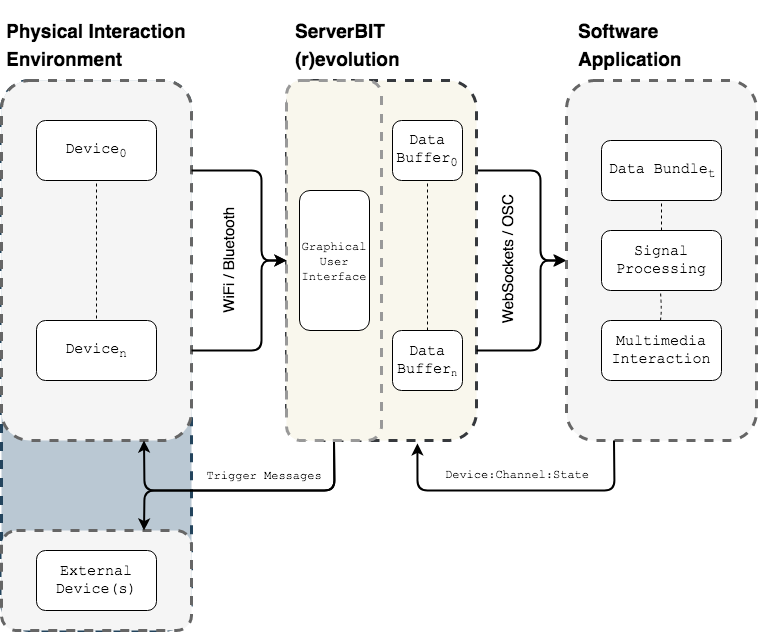
\includegraphics[width=\textwidth]{Chapters/Figures/technical/ServerBIT/ServerBIT_Archietecture_EXT.png}
    \caption{Overview of the ServerBIT Architecture}
    \label{fig:diagram1}
\end{figure}

\section{Design Principles}

\paragraph{Sequential Data Format}
Data buffers provide information regarding how a signal behaves over a given time period. Sensor data is received as a bundle containing an array of contiguous float values for each channel, where the most recent reading is given at the head of the buffer. The proposed ServerBIT development pipeline provides a convenient format for data visualisation and digital signal processing by granting users access to the entire frame buffer.

\paragraph{Open Source}
Users should acknowledge that they can make full use of the provided examples without needing to access the ServerBIT source code. Nonetheless, if a user intends to re-purpose the software to satisfy their specific project, it may be necessary to alter certain components of the script. Some reasons for this might include: adding support for additional hardware devices, pre-processing signals before forwarding to external applications or integrating functionality from additional libraries. With this considered, the source code is openly available to the public, including instructions on compiling and running the application from the user's command line.

\paragraph{Automatic Device Connection and Re-connection Handling}
When new users try to incorporate sensor-based interaction, a considerable technical barrier has their application successfully recognise the device connection. In a rapid prototyping environment, users are susceptible to more issues as they wish to experiment with different device configurations. Matters can worsen when using multiple devices, particularly when each relies on different communication technologies. For example, the BITalino requires either standard Bluetooth or BLE, whereas the R-IoT device communicates over WiFi. When a connection drops, the application as a whole may fail to operate and troubleshooting the specific issue can be onerous to those unfamiliar with the hardware.

\begin{figure}[htb!]
    \centering
    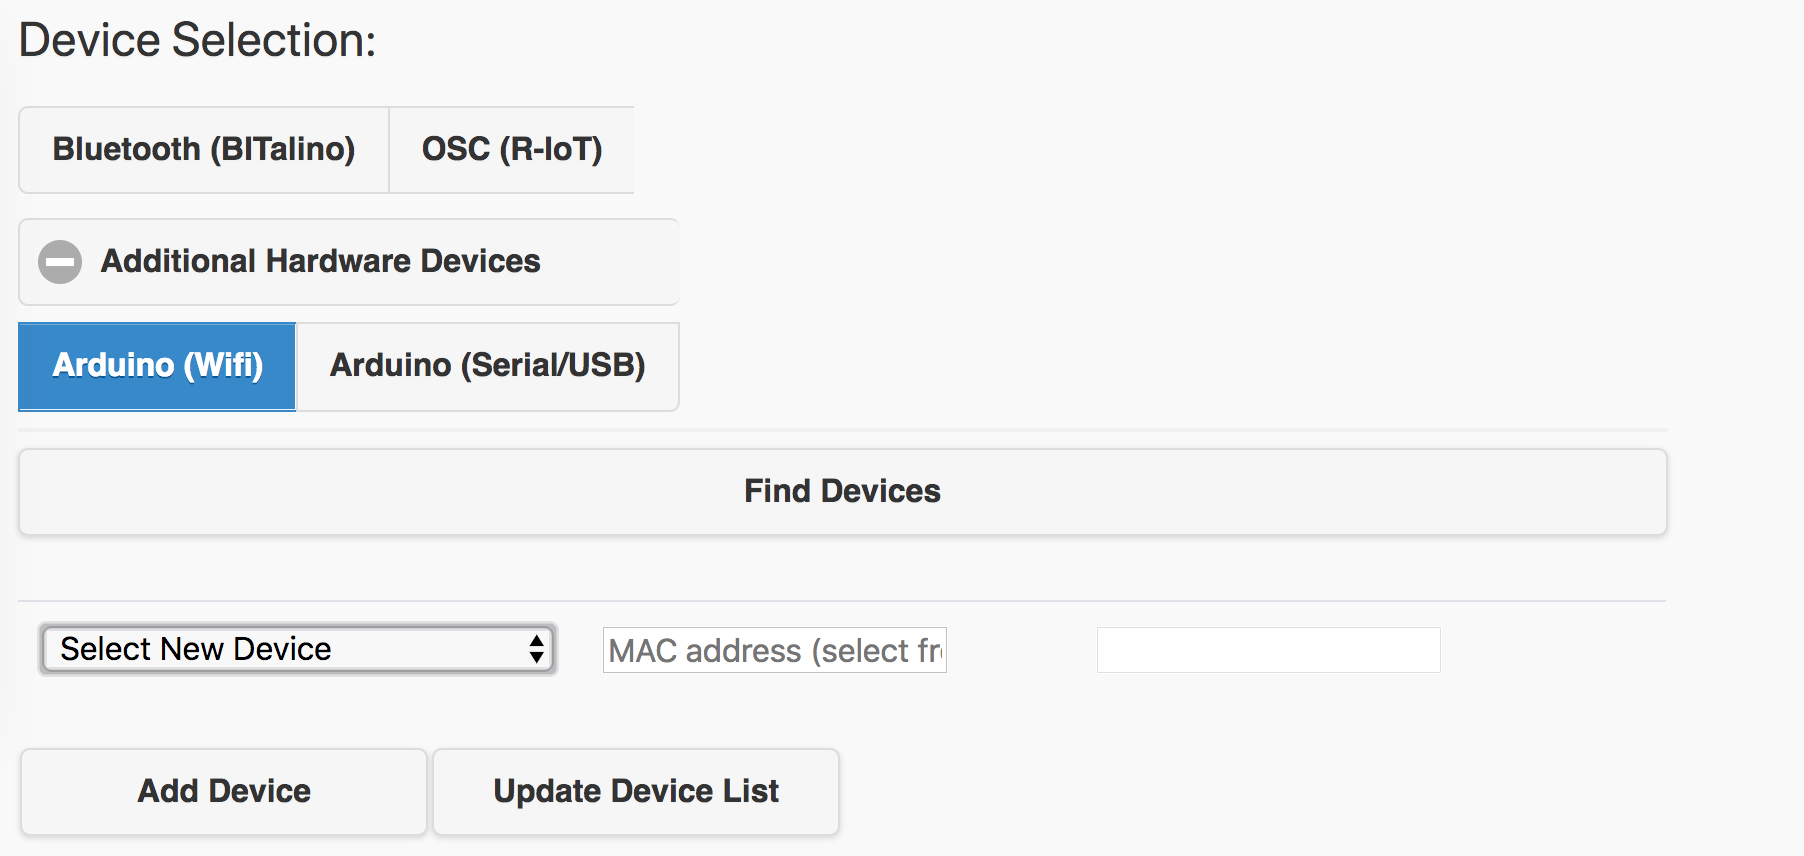
\includegraphics[width=100mm,scale=1.0]{Chapters/Figures/technical/ServerBIT/device_selection.png}
    \caption{ServerBIT configuration page.}
    \label{fig:dev_selection}
\end{figure}

On the configuration page presented in Fig. \ref{fig:dev_selection}, users can use the device finder menu, which searches for available serial, Bluetooth and Wi-Fi connections nearby. From here, users are presented with an accumulation of device addresses, which can be added to ServerBIT's device list. When the configuration is successfully updated, ServerBIT will automatically attempt to establish a new connection with each device in the list.

\paragraph{Physiological Data Transmission Over Wi-Fi} \label{riot}

ServerBIT is designed to be compatible with BITalino R-IoT devices, which transmit multiple data channels over a local Wi-Fi network. This alternative to Bluetooth-based communication holds several advantages. However, it necessitates for the user to set the IPv4 address of their computer to a specific static IP address. For users unfamiliar with this process, this will likely increase the burden of pairing new devices, thus interrupting application development. Before searching for new devices, ServerBIT will detect the current network configuration and generate a shell or bash command according to the operating system. The command can be validated and executed with the graphical interface. Upon execution, ServerBIT matches the computer's IPv4 address accordingly with the module's destination address.

\begin{figure}[ht]
    \centering
    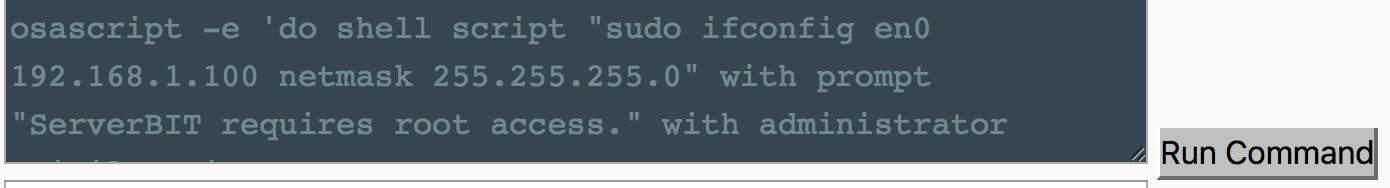
\includegraphics[width=\textwidth]{Chapters/Figures/technical/ServerBIT/ipv4_cmd_osx.png}
    \caption{Network command generated and displayed in the browser (MacOS)}
    \label{fig:cmd_osx}
\end{figure}

\paragraph{Uninterrupted Hardware Connections During Development}

A trigger handler is automatically established and initiated for each device added to the network. The trigger handler runs in the background and listens for OSC messages addressed in the following format "/\textbf{deviceID/output"}. These messages authorise control of the separate digital and analog outputs on individual or multiple devices. This bidirectional communication intends to support interactive systems design where biofeedback mechanisms respond to physiological input in real-time. This approach can also be used to send commands to WiFi-enabled devices, bypassing the labour of bridging the devices over a wired serial connection.

\paragraph{Biofeedback Control Using OSC} \label{Biofeedback}

For each device added to the network, a trigger handler is automatically established and initiated. The trigger handler runs in the background and listens for OSC messages addressed in the following format \textit{"/\textbf{deviceID}/output"}. These messages authorise control of the separate digital and analog outputs on individual or multiple devices. This bidirectional communication intends to support the design of interactive systems where biofeedback mechanisms respond to physiological input in real-time. This approach can also be used to send commands to WiFi-enabled devices, bypassing the labour of bridging the devices over a wired serial connection.

\section{Running A ``Hello World'' Example}

\paragraph{Pairing a New Device} \label{Pairing}
In the case of BITalino, every device has a unique hardware address that must be declared within ServerBIT. On the configuration page (Fig. \ref{fig:dev_selection}), users are presented with a list of device addresses that have already been paired with the host computer. One or more devices can be selected from the list, and upon submission, ServerBIT will begin to read sensor data from each module respectively.

\paragraph{Data Acquisition}
Once a device has been paired, the user can determine which channels will be acquired and modify the format in which they will be transmitted. In order to run this first example, the user does not need to make any changes here, as the default configuration is already set up to read and stream data from the first analogue input labelled \textbf{'A1'}.

\paragraph{Network Settings}
At the bottom of the configuration page, the user can specify the network protocol for communicating with the interactive application layer. By default, ServerBIT is set to stream sensor data to a local server (\textit{127.0.0.1} or \textit{localhost}) over the WebSocket protocol using the port number 8000; this configuration can be used with the web-based examples provided in the software package.

\paragraph{ClientBIT Example}
Provided within the ServerBIT package is a basic example that can be used to test the connection to a BITalino device and visualise an incoming signal on the browser. \textit{ClientBIT.html} is an example HTML/JS
test client which prompts the back end to initialise a connection to a specified BITalino device. Once a connection is established from host to client, sensor data is acquired from channel \textbf{'A1'} and plotted in real-time. The HTML file can be found in the ServerBIT directory, located inside the user's home folder, which also includes the \textit{jquery} library files required to run the example.

\begin{figure}[htb!]
    \centering
    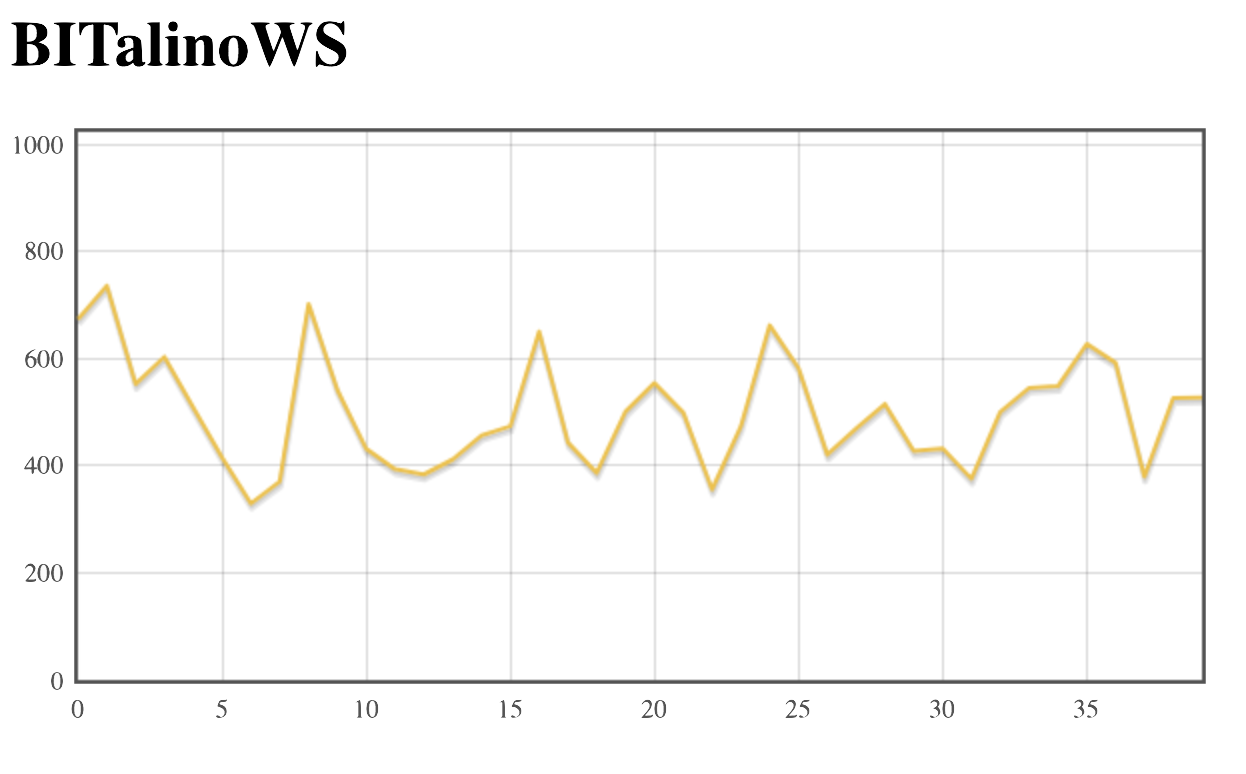
\includegraphics[width=65mm,scale=0.65]{Chapters/Figures/technical/ServerBIT/ClientBIT_html.png}
    \caption{ClientBIT.html displaying an EMG signal in the browser}
    \label{fig:ClientBIT}
\end{figure}
%\subsection{Controlling Applications with Multiple Devices}

\section{Exporting and Sharing Applications}

\paragraph{Portable Configurations}

When attempting to distribute example applications to new users, we often perceive difficulties where additional configuration tasks are required to run the application. This process can be inefficient when involving many participants or even remote scenarios, particularly when dealing with users unfamiliar with the specific technologies and software libraries.

A major goal of ServerBIT was to improve the portability of sensor-based applications. For this to be satisfied, it should be possible for new users to receive a software package that can be executed on their machine without the need to make changes to the source code. At a minimum, such a software package should include (1) the ServerBIT executable, (2) the source code for the application that handles the incoming data, and (3) a preset configuration file that can be imported with the ServerBIT GUI.

\paragraph{Saving a Preset}

The ServerBIT configuration page is accessible from a web browser. When accessing the page for the first time, the user is presented with the default settings. In order to interact with the software, the user must select and pair at least one new device (see Section \ref{Pairing}). When completed, clicking \textbf{"Submit"} at the bottom of the form will save the current configuration into the ServerBIT home directory as \textit{config.json}.

\begin{figure}[htb!]
    \centering
    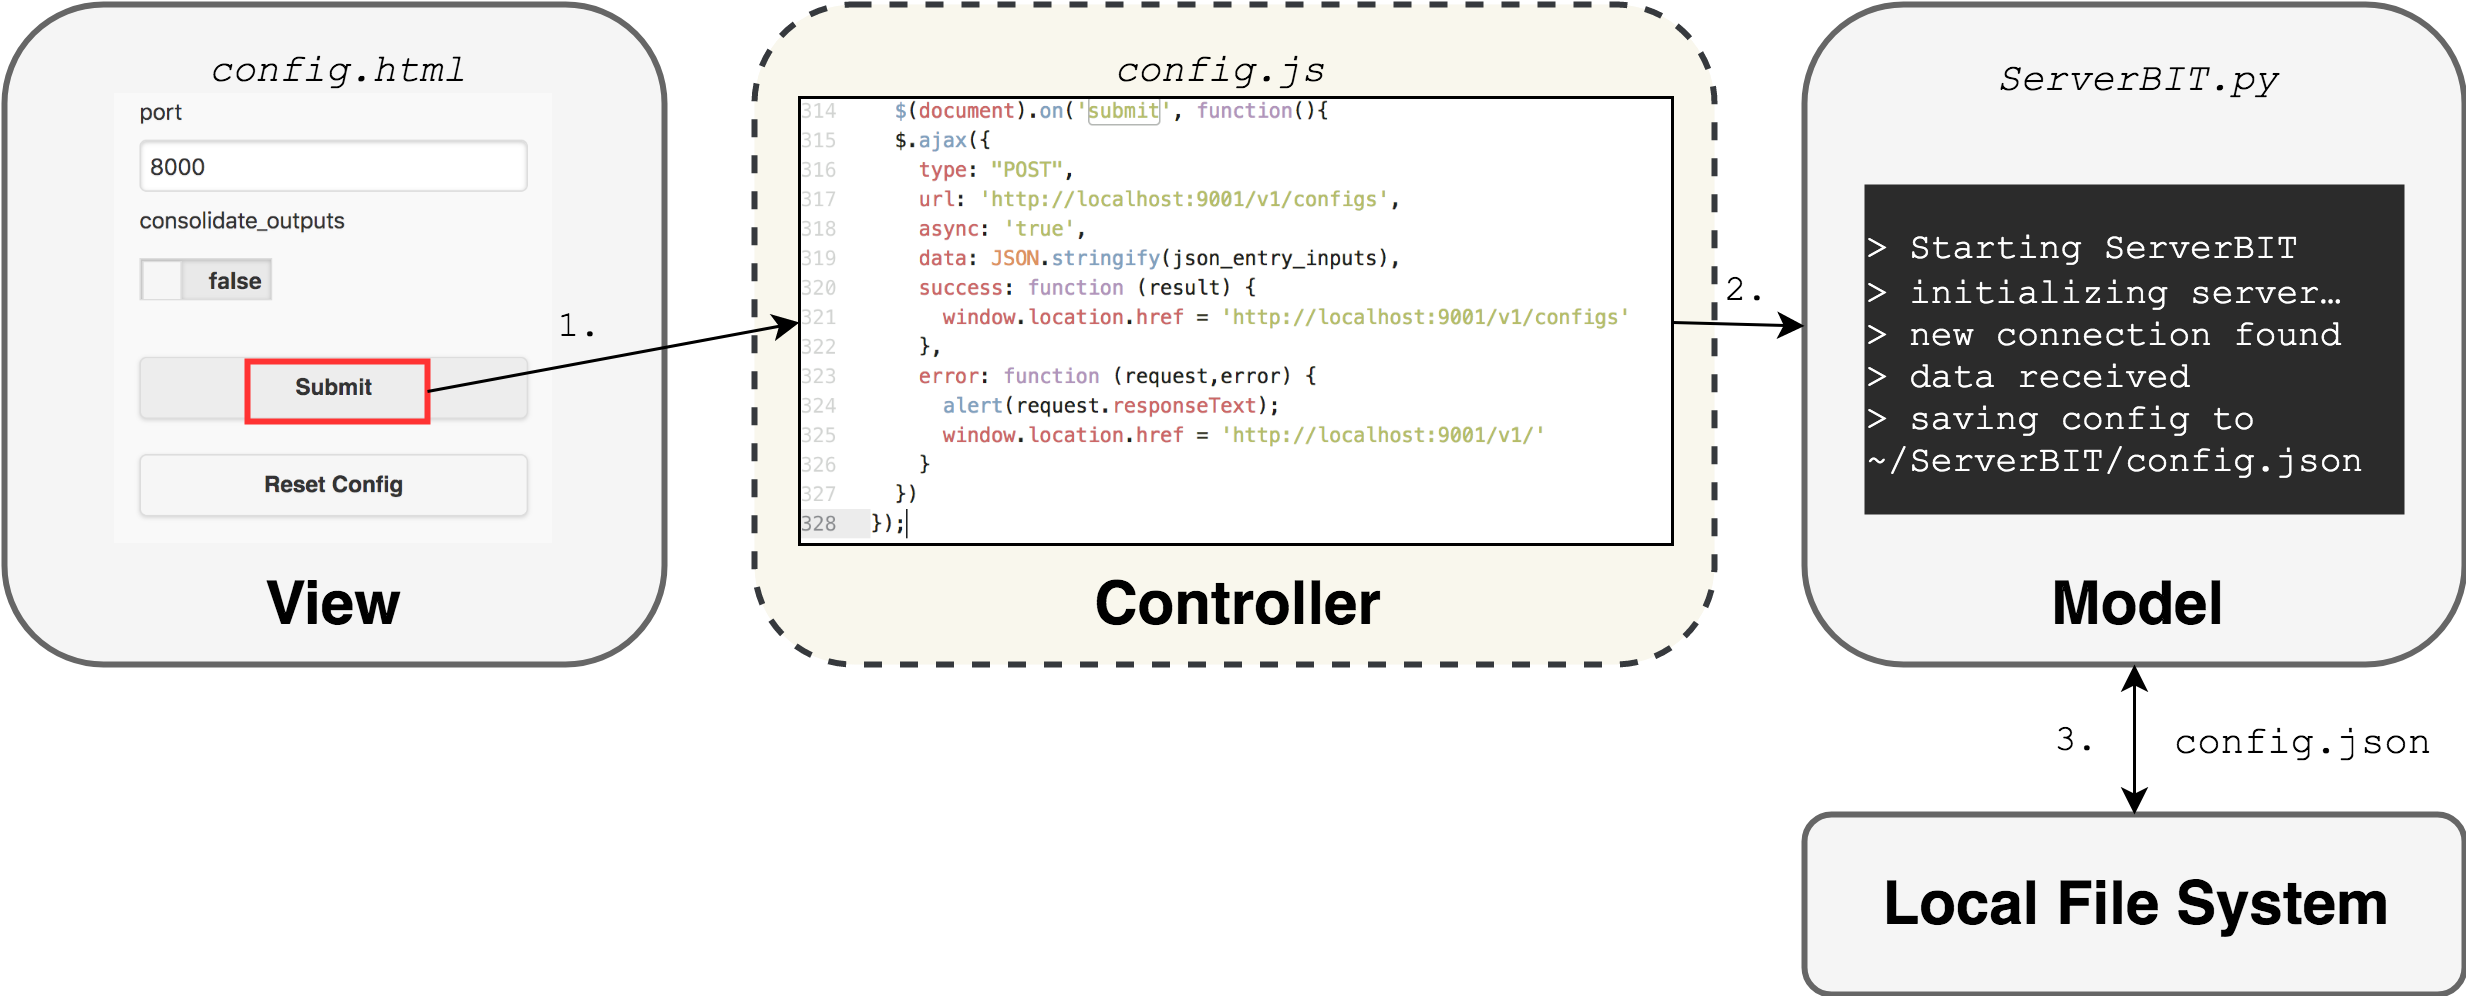
\includegraphics[width=\textwidth]{Chapters/Figures/technical/ServerBIT/Websockets_ctrl.png}
    \caption{Workflow of the configuration saving process}
    \label{fig:MVC_Diagram}
\end{figure}

% \newpage
This micro-framework was designed under a Model-View-Controller (MVC) architecture. A Python WebSocket server communicates between the presentation layer and the processing and persistency layers \cite{da_silva_web-based_2012}. The unified process can be separated into three interdependent modules, as shown in Figure \ref{fig:MVC_Diagram}, authorising access to network properties and low-level hardware specificities from a visual interface.

\paragraph{Loading an Existing Configuration File}

From the browser interface, users can import an existing configuration file in ServerBIT's JSON format. The new settings, such as device addresses and channel labels, will be displayed as form entries; these can be altered accordingly and saved by re-submitting the form.

Users should note that for the sensor data to reach a new OSC or WebSocket listener, the port number and host IP address must match what's assigned to the ServerBIT configuration. If these parameters are changed from their defaults, they should be saved to the configuration file so the sensor data can stream to the server upon launching without issues.

\section{Summary}

In this chapter, we presented ServerBIT (r)evolution, a software toolkit serving to complete the interaction loop between sensory hardware devices and multimedia applications, including those that can be run on a web browser. We provide a brief overview of existing utilities, which deliver a comparable service of abstracting hardware-specific configurations within a rapid-prototyping scenario. From this, we formulate criteria for a set of software requirements based on the common issues developers experience when prototyping new interaction modalities with physiological sensors; this is used to justify our design choices which are subsequently described throughout the report.
 % Three specialist use-cases are reviewed to demonstrate some of the prototyping capabilities that go beyond what was provided in the previous iterations of ServerBIT.
Proposed future work will consider the evaluation of the toolkit as an educational tool, with ambitions to introduce sensor-based applications to new communities that specialise in other technical domains. Such field-work opportunities will advocate for the assessment of user feedback to discover in what scenarios this approach is potentially advantageous and later warrant new adaptations of the toolkit in forthcoming iterations.
